\documentclass[border=12pt]{standalone}
\def\pgfsysdriver{pgfsys-dvisvgm.def}
\usepackage[dvisvgm]{xcolor}
\usepackage{xeCJK}
\setCJKmainfont{HaranoAjiGothic-Regular.otf}[BoldFont=HaranoAjiGothic-Bold.otf]
\setCJKsansfont{HaranoAjiGothic-Regular.otf}[BoldFont=HaranoAjiGothic-Bold.otf]
\usepackage{amsmath,amssymb,tikz,lmodern}
\usetikzlibrary{arrows.meta,positioning,calc,fit,backgrounds}
\renewcommand{\familydefault}{\sfdefault}
\definecolor{ink}{HTML}{25322F}
\definecolor{green}{HTML}{246657}
\definecolor{tint}{HTML}{EEF4F0}
\definecolor{soft}{HTML}{C6D2CC}
\definecolor{muted}{HTML}{52615B}
\newif\ifJapanese
\newcommand{\Tx}[2]{\ifJapanese #1\else #2\fi}
\newcommand{\Eff}{\overline{\operatorname{Eff}}}
\newcommand{\heading}[3]{{\color{green}\bfseries #1\quad\Tx{#2}{#3}}\\[5pt]}
% A white rectangle makes the complete citation label clickable, including spaces.
\newcommand{\refurl}[2]{\special{dvisvgm:raw <a xlink:href="#1" target="_blank" rel="noopener noreferrer">}{\setlength{\fboxsep}{0pt}\colorbox{white}{\color{green}\underline{\strut #2}}}\special{dvisvgm:raw </a>}}
\tikzset{
 card/.style={draw=soft,fill=white,rounded corners=2pt,align=left,text=ink,font=\fontsize{10.5}{14}\selectfont,inner xsep=12pt,inner ysep=10pt,text width=14.4cm},
 half/.style={card,text width=6.45cm,minimum height=2.05cm},
 result/.style={card,draw=green,fill=tint,line width=.9pt},
 reason/.style={align=left,text=muted,font=\fontsize{9}{12}\selectfont,inner sep=0pt,text width=12.7cm},
 branchreason/.style={reason,text width=5.95cm},
 edge/.style={-{Stealth[length=2.4mm]},draw=green,line width=1pt},
 wire/.style={draw=green,line width=1pt},
}
% Keep the arrow in a dedicated left gutter; explanations never cover it.
\newcommand{\flow}[3]{
 \coordinate (#2-from) at ($(#1.south)+(-6.9,0)$);
 \coordinate (#2-to) at ($(#2.north)+(-6.9,0)$);
 \draw[edge] (#2-from)--(#2-to);
 \node[reason,anchor=west] (#2-reason) at ($(#2-from)!.5!(#2-to)+(.55,0)$) {#3};
}

\newcommand{\Cite}[2]{\refurl{#1}{#2}}

\Japanesefalse
\begin{document}
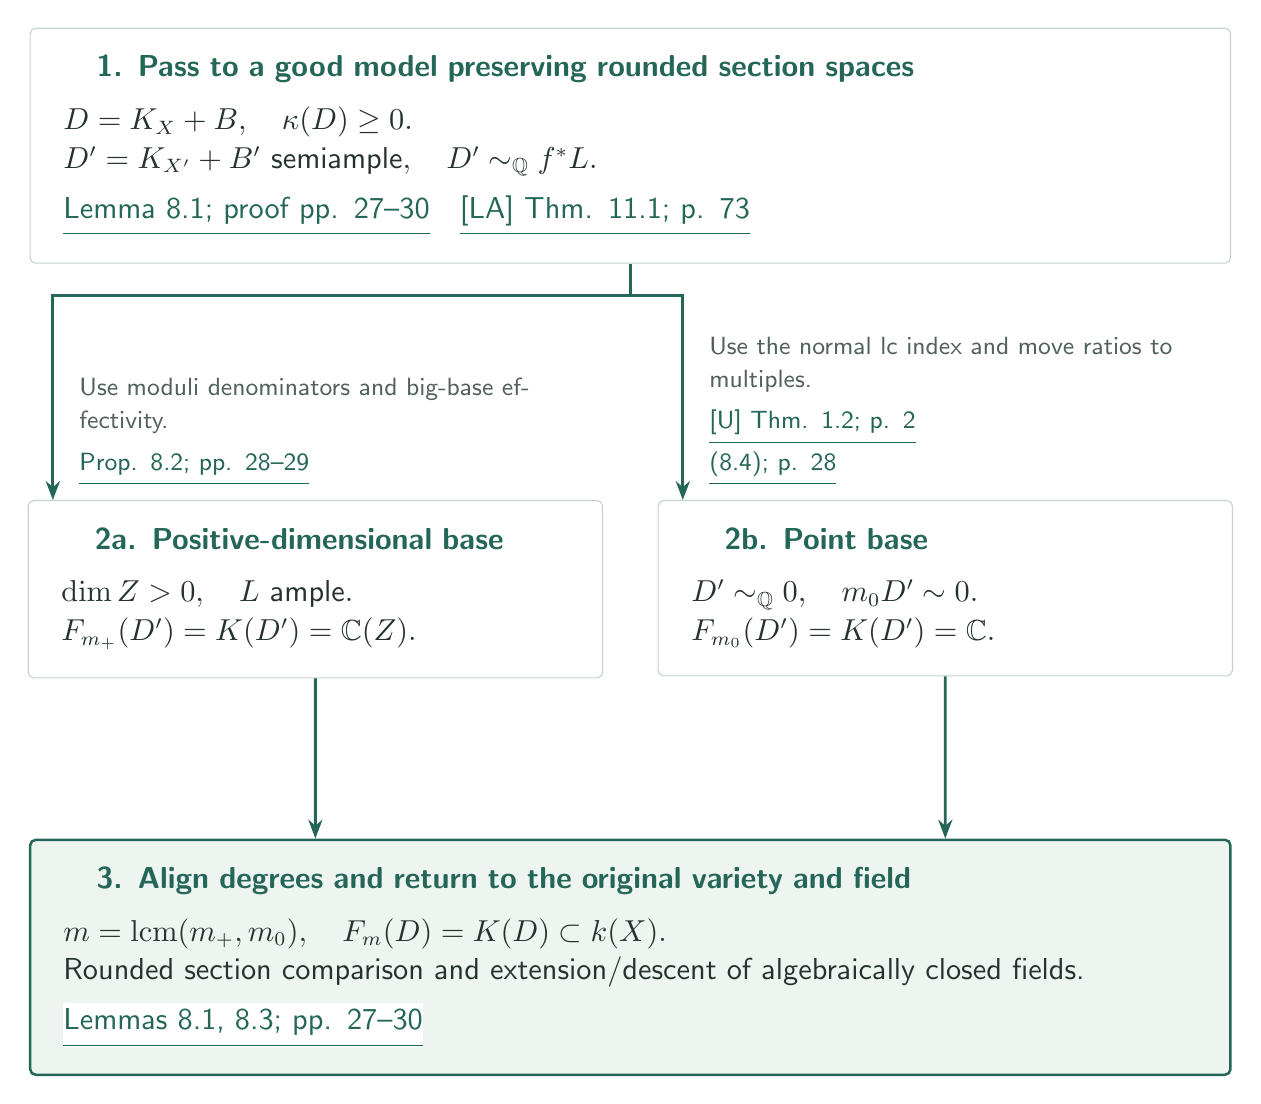
\begin{tikzpicture}
\node[card] (model) {\heading{}{1. 丸めた切断空間を保ってgood modelへ}{1. Pass to a good model preserving rounded section spaces}$D=K_X+B,\quad\kappa(D)\ge0.$\\ $D^{\prime}=K_{X^{\prime}}+B^{\prime}\text{ semiample},\quad D^{\prime}\sim_{\mathbb Q}f^*L.$\\[4pt]\Cite{https://github.com/openai/math/blob/adc7f1241b42e322a6451854ab7e4b4c146bf78a/preprints/Uniform-log-Iitaka-fibrations-and-bounded-moduli-denominators-October-4-2026/uniform-log-iitaka.pdf}{Lemma 8.1; proof pp. 27--30}\quad \Cite{https://github.com/openai/math/blob/adc7f1241b42e322a6451854ab7e4b4c146bf78a/preprints/Log-abundance-in-characteristic-zero-September-24-2026/paper.pdf}{[LA] Thm. 11.1; p. 73}};

\node[half,below=3cm of model.south,xshift=-4cm] (positive) {\heading{}{2a. 底が正次元}{2a. Positive-dimensional base}$\dim Z>0,\quad L\text{ ample}.$\\ $F_{m_+}(D^{\prime})=K(D^{\prime})=\mathbb C(Z).$};

\node[half,below=3cm of model.south,xshift=4cm] (zero) {\heading{}{2b. 底が点}{2b. Point base}$D^{\prime}\sim_{\mathbb Q}0,\quad m_0D^{\prime}\sim0.$\\ $F_{m_0}(D^{\prime})=K(D^{\prime})=\mathbb C.$};

\coordinate (positive-a) at ($(positive.north west)+(.32,0)$);
\draw[edge] (model.south) -- ++(0,-.4) -| (positive-a);
\node[branchreason,anchor=south west] at ($(positive.north west)+(.65,.18)$) {\Tx{moduli分母とbigな底の有効性を使う。}{Use moduli denominators and big-base effectivity.}\\[3pt]\Cite{https://github.com/openai/math/blob/adc7f1241b42e322a6451854ab7e4b4c146bf78a/preprints/Uniform-log-Iitaka-fibrations-and-bounded-moduli-denominators-October-4-2026/uniform-log-iitaka.pdf}{Prop. 8.2; pp. 28--29}};

\coordinate (zero-a) at ($(zero.north west)+(.32,0)$);
\draw[edge] (model.south) -- ++(0,-.4) -| (zero-a);
\node[branchreason,anchor=south west] at ($(zero.north west)+(.65,.18)$) {\Tx{normal lc指数と、切断比の倍数移送。}{Use the normal lc index and move ratios to multiples.}\\[3pt]\Cite{https://github.com/openai/math/blob/adc7f1241b42e322a6451854ab7e4b4c146bf78a/preprints/Uniform-Pluricanonical-Iitaka-Fibrations-October-3-2026/paper.pdf}{[U] Thm. 1.2; p. 2}\\ \Cite{https://github.com/openai/math/blob/adc7f1241b42e322a6451854ab7e4b4c146bf78a/preprints/Uniform-log-Iitaka-fibrations-and-bounded-moduli-denominators-October-4-2026/uniform-log-iitaka.pdf}{(8.4); p. 28}};

\node[result,below=7.3cm of model.south] (end) {\heading{}{3. 次数を合わせ、元の多様体と体へ戻す}{3. Align degrees and return to the original variety and field}$m=\operatorname{lcm}(m_+,m_0),\quad F_m(D)=K(D)\subset k(X).$\\ \Tx{丸めた切断比較と、代数閉体の拡大・降下。}{Rounded section comparison and extension/descent of algebraically closed fields.}\\[4pt]\Cite{https://github.com/openai/math/blob/adc7f1241b42e322a6451854ab7e4b4c146bf78a/preprints/Uniform-log-Iitaka-fibrations-and-bounded-moduli-denominators-October-4-2026/uniform-log-iitaka.pdf}{Lemmas 8.1, 8.3; pp. 27--30}};

\draw[edge] (positive.south) -- ($(end.north)+(-4,0)$);
\draw[edge] (zero.south) -- ($(end.north)+(4,0)$);
\end{tikzpicture}
\end{document}
